\documentclass[12pt,a4paper]{article}
\usepackage{graphicx}
\usepackage[english,ngerman]{babel}
\usepackage[parfill]{parskip} % to start each parapraph will an empty line before
\usepackage{listings}
\usepackage{hyperref}
\usepackage{float}

\begin{document}
	\begin{titlepage}
		\centering
		
\includegraphics[width=0.8\textwidth]{img/Hska_logo.png}\par\vspace{1cm}
		{\scshape\LARGE Dokumentation\par}
		\vspace{1.5cm}
		{\huge\bfseries Verteilte Systeme Master Labor\par}
		\vspace{2cm}
		{\Large\itshape Pol Zeimet (65834) \\\href{mailto:zepo1012@hs-karlsruhe.de}{zepo1012@hs-karlsruhe.de}\par}
		\vfill
		{\Large\itshape Yannick Stephan (65934) \\\href{mailto:stya1012@hs-karlsruhe.de}{stya1012@hs-karlsruhe.de}\par}
		\vfill
		\large Aufgabe 2
		
		\vfill
		
		% Bottom of the page
		{\large \today\par}
	\end{titlepage}
	\section{Architekturentwurf}
	\label{sec:Architekturentwurf}
		Auf Basis der Analyse aus Aufgabe 1 wurde eine Microservice Architektur entworfen, welche in Abbildung \ref{fig:microservices-architecture} zu sehen ist. Diese Architektur beinhaltet eine Menge von Core-, Composite- und API-Services. Eine genauere Beschreibung der einzelnen Services sind in den folgenden Unterkapiteln zu entnehmen. In Kapitel 2 sind die konkreten REST-API Schnittstellen der einzelnen Services aufgezeigt.
		
		\begin{figure}[H]
			\centering
			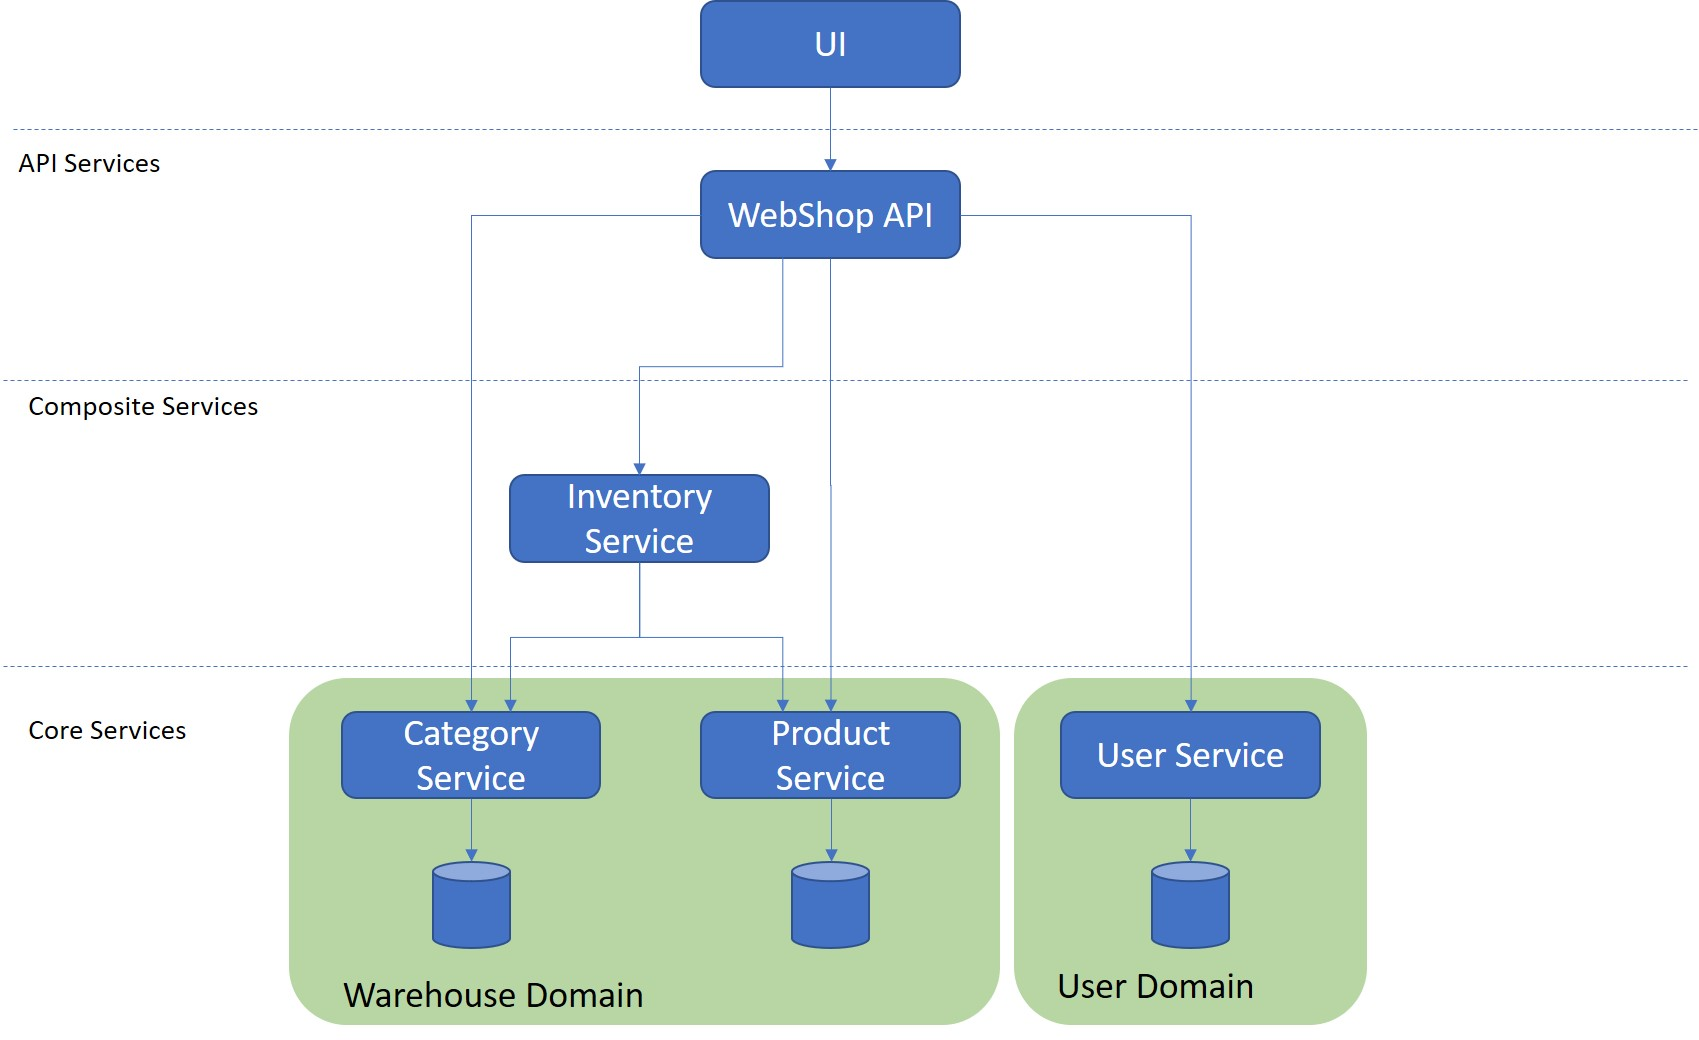
\includegraphics[scale=0.45]{diagrams/microservices-architecture.jpg}
			\caption{Entwurf einer Microservice-basierten Zielarchitektur}
			\label{fig:microservices-architecture}
		\end{figure}
	
		\subsection{API Services}
			\subsubsection{WebShop API}
			Dieser API-Service dient als Schnittstelle zwischen der Frontend-Anwendung und den restlichen Microservices, die von außen nicht sichtbar sein sollen.
			
		\subsection{Composite Service}
			\subsubsection{Inventory Service}
			Der Inventory Service ist für alle Funktionen zuständig, bei denen es Abhängigkeiten zwischen Produkten und Kategorien gibt.
		
		\subsection{Core Services}
			\subsubsection{Category Service}
			Der Category Service erstellt, löscht und listet Kategorien der WebShop-Anwendung.
			
			\subsubsection{Product Service}
			Der Product Service ist für das Listen, Erstellen und Suchen von Produkten der Anwendung zuständig.
			
			\subsubsection{User Service}
			Der User Service ist zuständig für die Benutzerverwaltung der Anwendung. Hier können neue Benutzer angelegt und ausgegeben werden. Zudem können sich Rollen anhand vom Benutzerlevel zurückgegeben werden lassen.
			
	\newpage
	\section{REST-API}
	\label{sec:REST-API}
	Alle yaml-Dateien für die folgenden REST-Schnitstellen befinden sich im Anhang.
	
	\subsection{WebShop API}
	\begin{figure}[H]
		\centering
		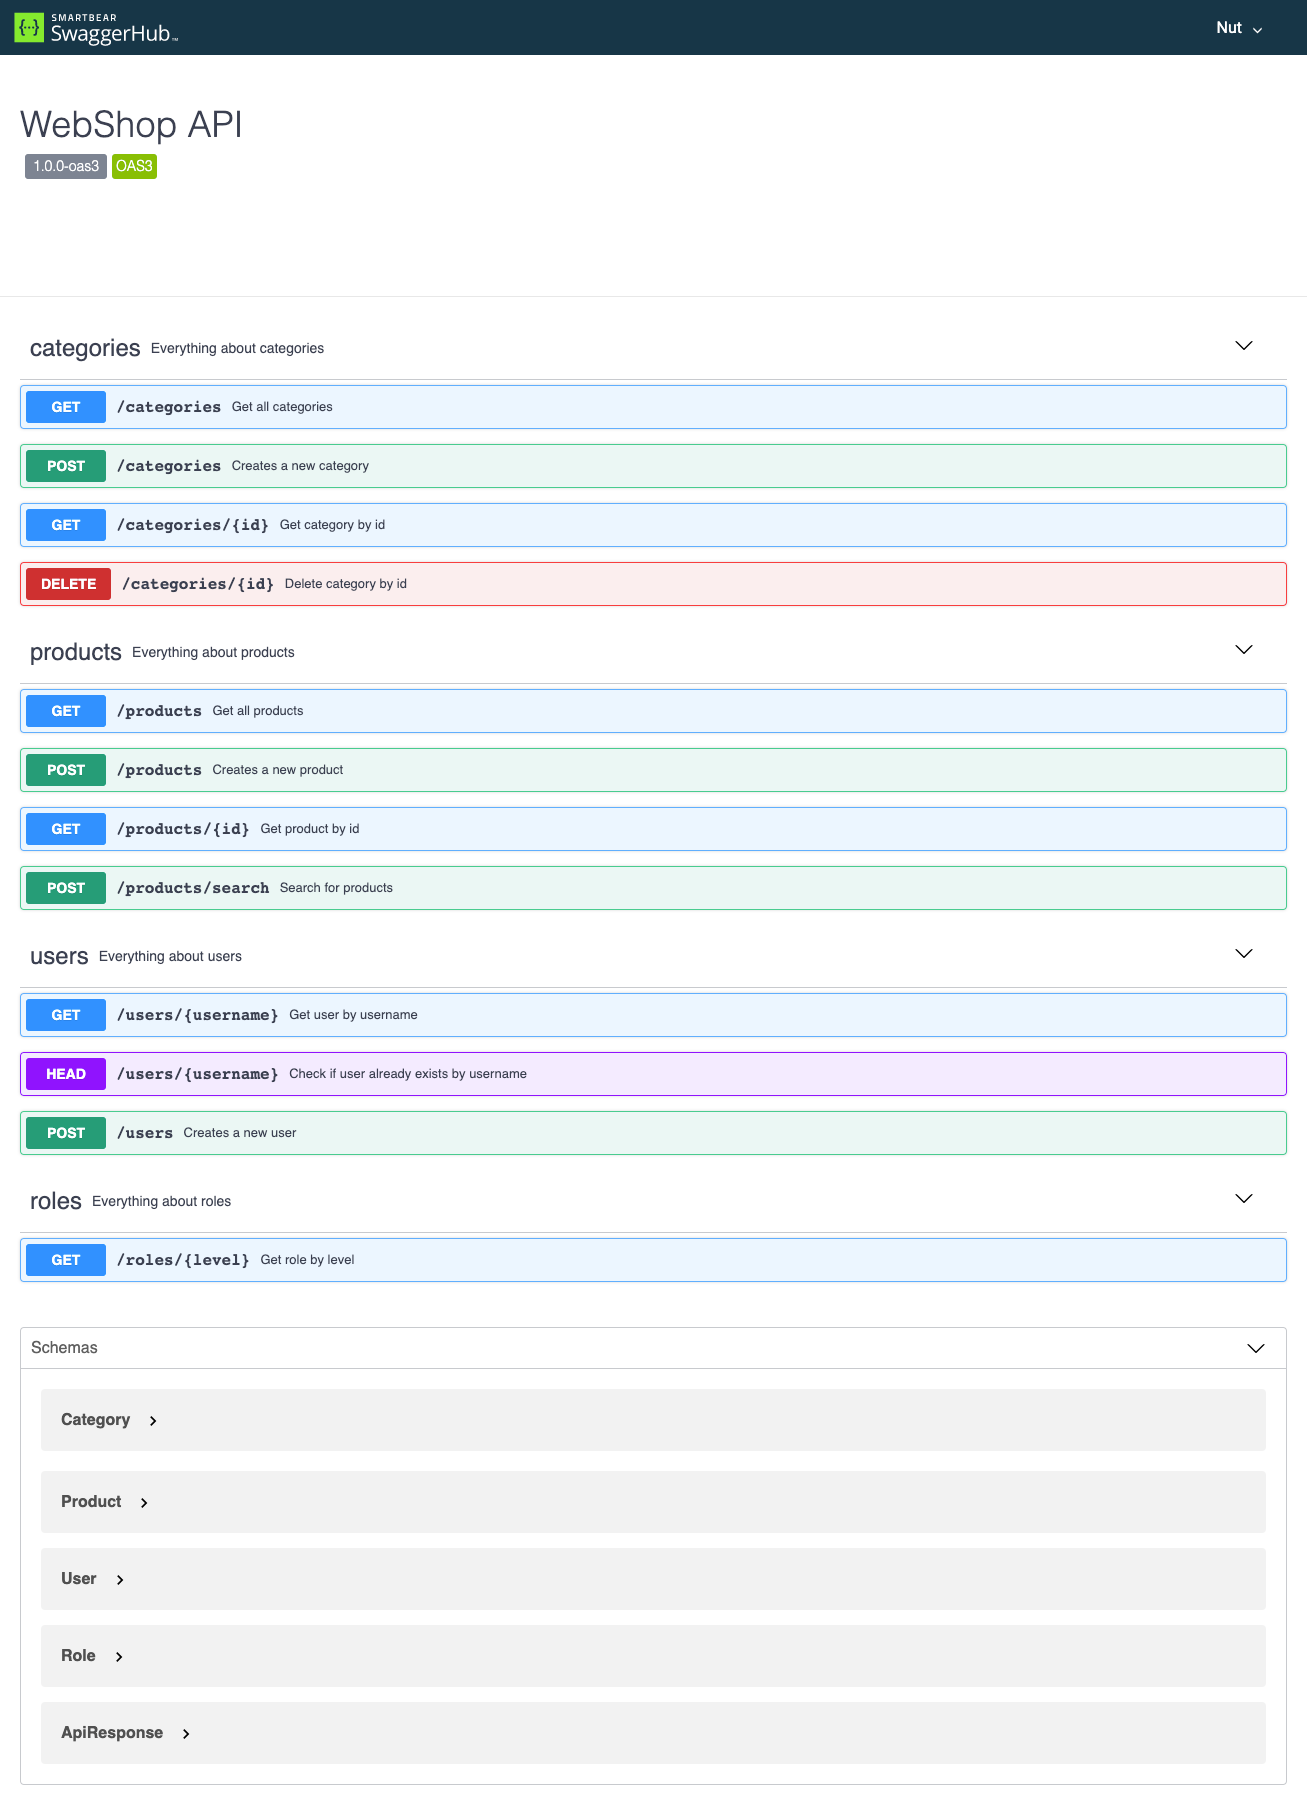
\includegraphics[scale=0.25]{img/swagger-webshop-api.png}
		\caption{WebShop REST-API}
	\end{figure}

	\subsection{Inventory Service API}
	\begin{figure}[H]
		\centering
		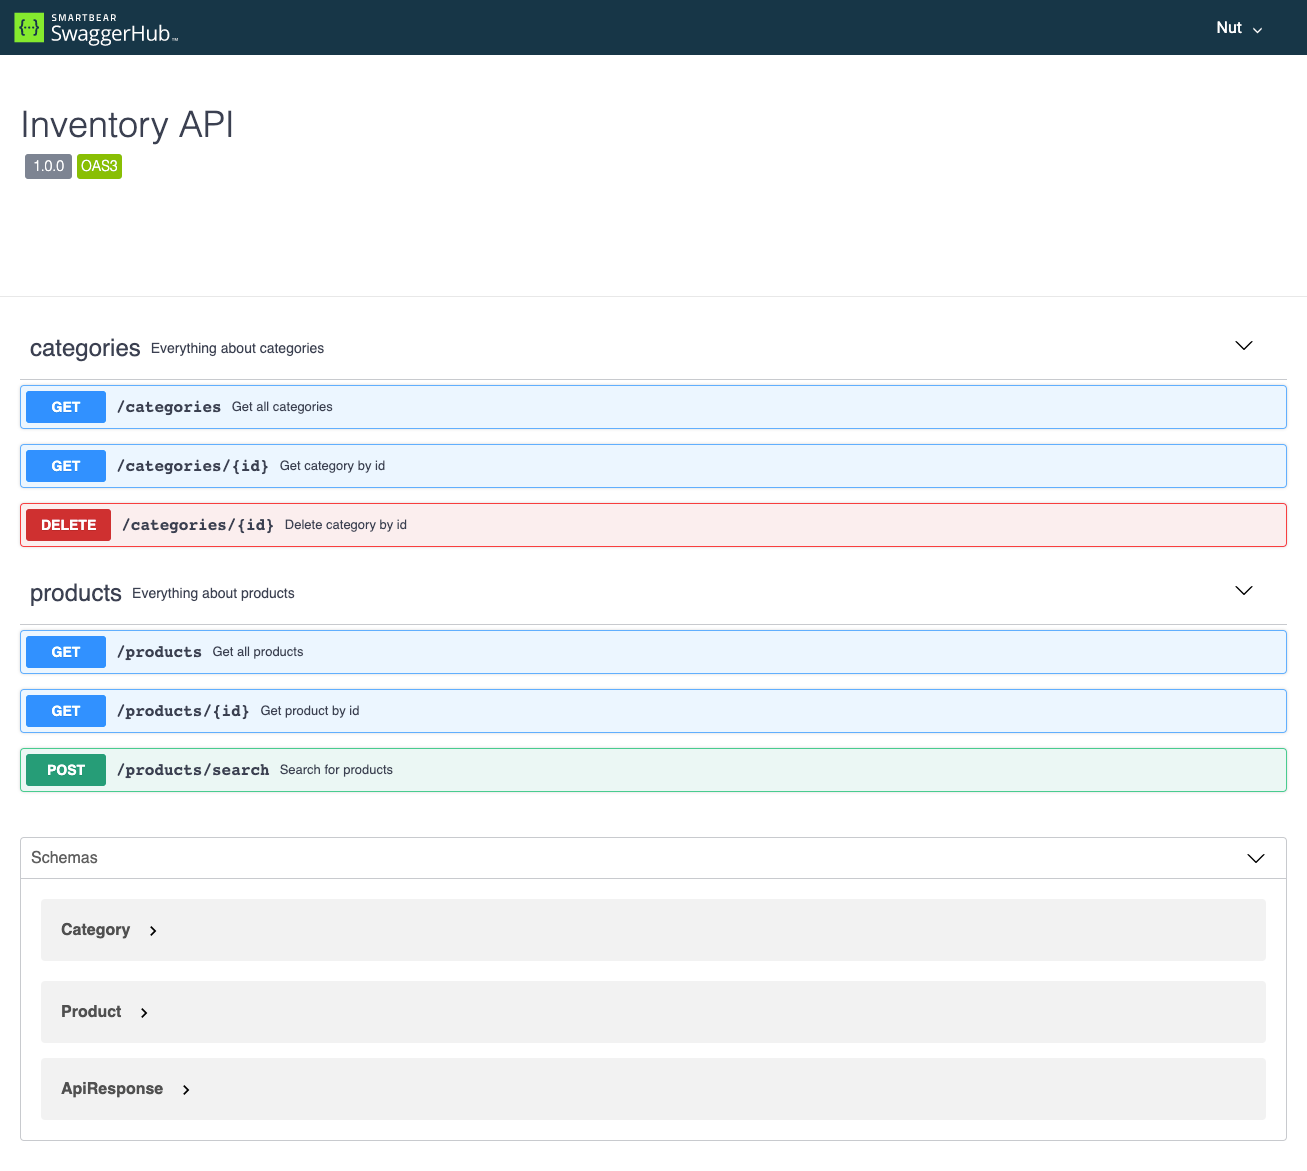
\includegraphics[scale=0.3]{img/swagger-inventory-service.png}
		\caption{Inventory Service REST-API}
	\end{figure}

	\subsection{Category Service API}
	\begin{figure}[H]
		\centering
		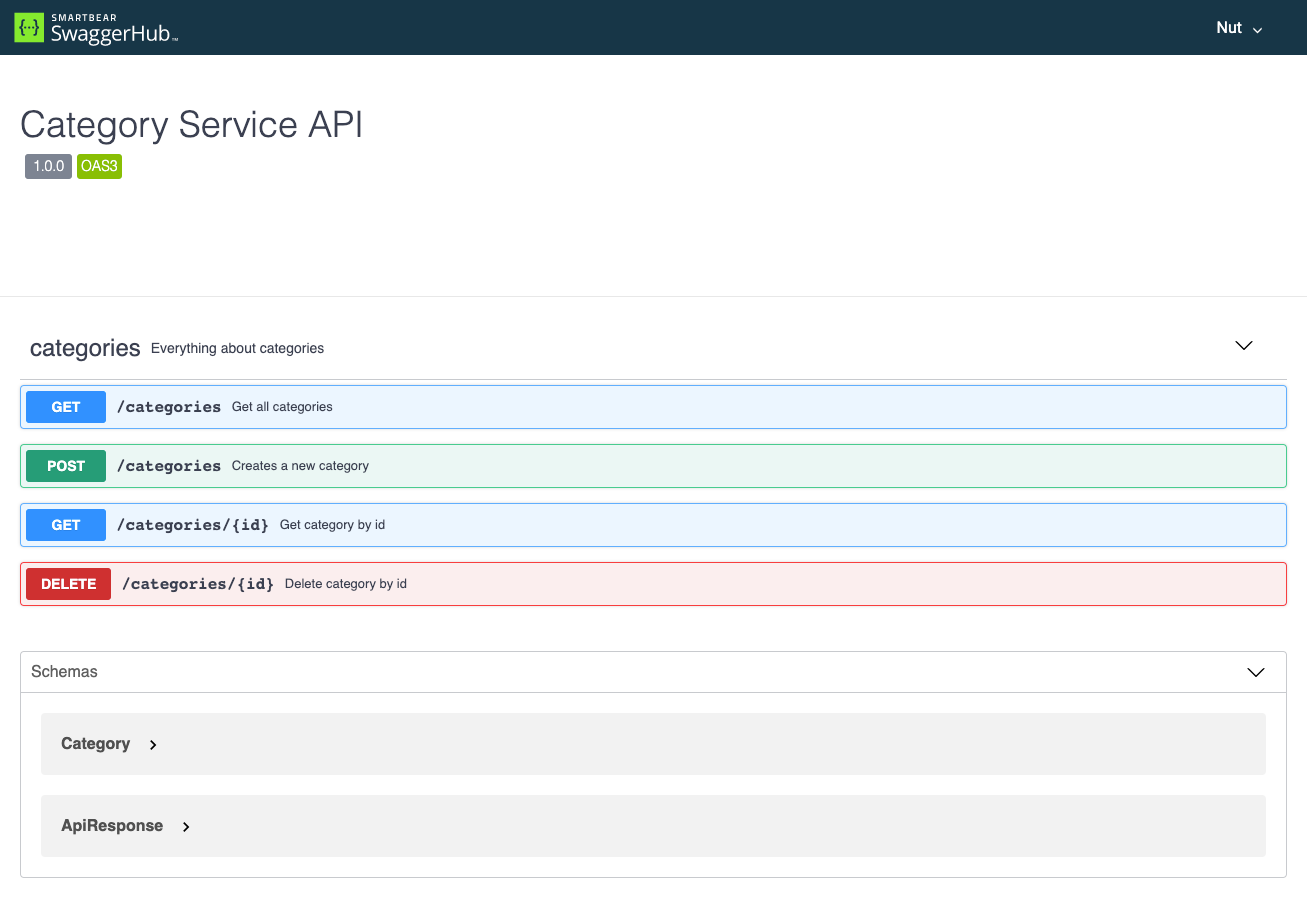
\includegraphics[scale=0.3]{img/swagger-category-service.png}
		\caption{Category Service REST-API}
	\end{figure}

	\subsection{Product Service API}
	\begin{figure}[H]
		\centering
		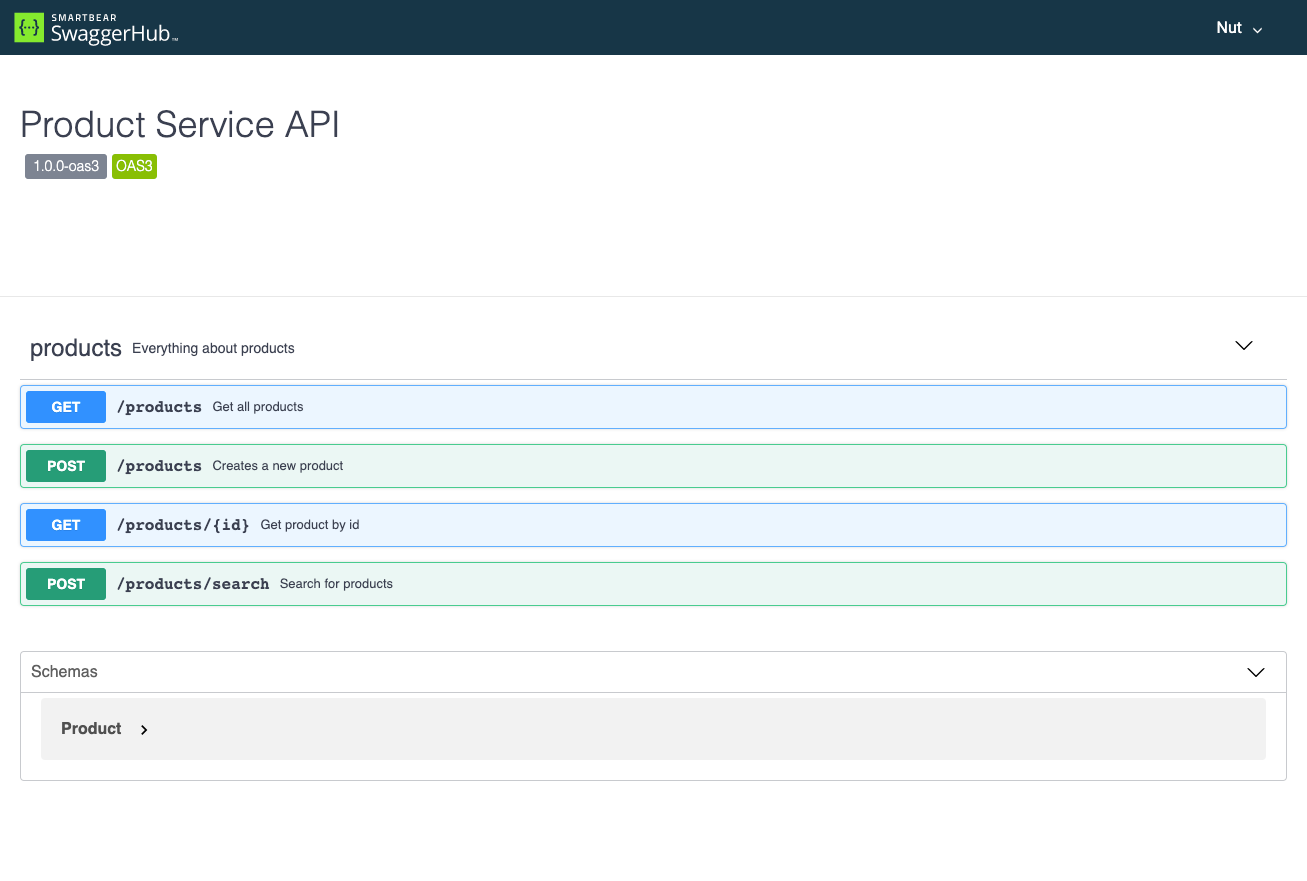
\includegraphics[scale=0.3]{img/swagger-product-service.png}
		\caption{Product Service REST-API}
	\end{figure}

	\subsection{User Service API}
	\begin{figure}[H]
		\centering
		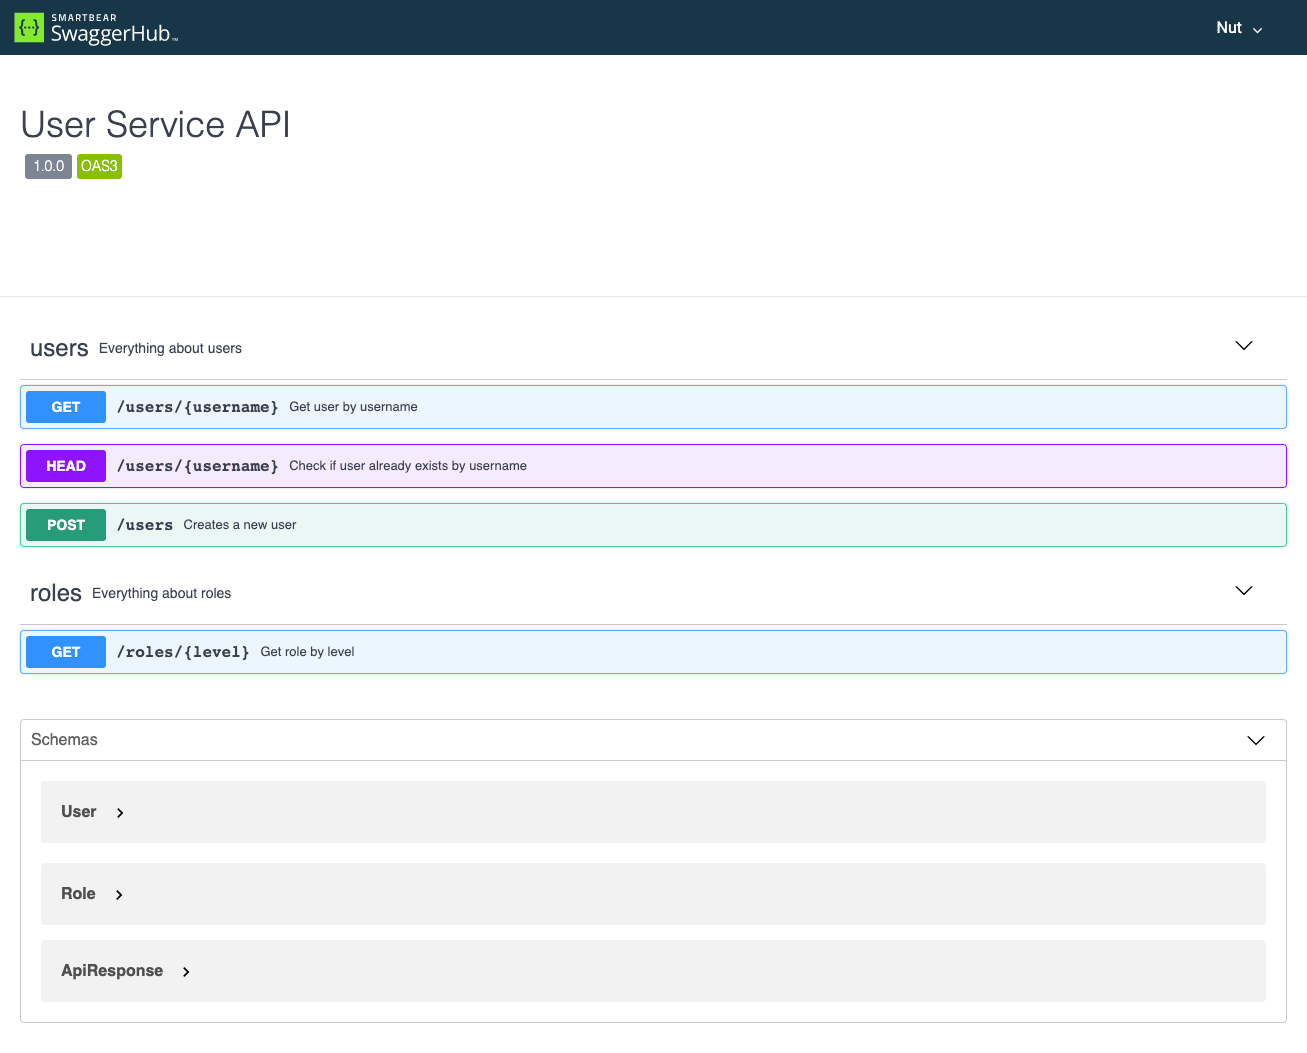
\includegraphics[scale=0.3]{img/swagger-user-service.png}
		\caption{User Service REST-API}
	\end{figure}
\end{document}